% !TeX program = pdflatex
% Build from the repository root; intermediates stay outside the source tree:
% ls /tmp/opencode
% mkdir -p /tmp/opencode/sticky-rod-document
% latexmk -pdf -interaction=nonstopmode -halt-on-error -file-line-error -outdir=/tmp/opencode/sticky-rod-document experiments/cu-cu-hybrid-bonding/1d-stickiness-model/model.tex
% cp /tmp/opencode/sticky-rod-document/model.pdf experiments/cu-cu-hybrid-bonding/1d-stickiness-model/model.pdf
\documentclass[11pt,a4paper]{article}
\usepackage[T1]{fontenc}
\usepackage{newtxtext,newtxmath}
\usepackage[margin=24mm,headheight=14pt]{geometry}
\usepackage{microtype}
\usepackage{amsmath}
\usepackage{booktabs,tabularx,array}
\usepackage{xcolor}
\usepackage{tikz}
\usetikzlibrary{arrows.meta,decorations.pathmorphing,patterns}
\usepackage{caption,fancyhdr,hyperref}
\definecolor{inkblue}{RGB}{36,64,87}
\hypersetup{colorlinks=true,linkcolor=inkblue,citecolor=inkblue,urlcolor=inkblue,
  pdftitle={A sticky elastic rod against a rigid wall},
  pdfsubject={Surviving-bond traction: rationale, equations, and implementation}}
\urlstyle{same}
\captionsetup{font=small,labelfont=bf}
\pagestyle{fancy}
\fancyhf{}
\fancyhead[L]{\small Sticky rod: formulation and implementation}
\fancyhead[R]{\small 6 September 2026}
\fancyfoot[C]{\small\thepage}
\renewcommand{\headrulewidth}{0.3pt}
\setlength{\parindent}{1.25em}
\setlength{\parskip}{0.25em}
\linespread{1.045}
\setlength{\emergencystretch}{1.5em}
\clubpenalty=10000
\widowpenalty=10000
\renewcommand{\arraystretch}{1.14}
\newcommand{\dd}{\mathrm{d}}
\newcommand{\code}[1]{\texttt{\detokenize{#1}}}
\newcommand{\pos}[1]{\left\langle #1\right\rangle_+}
\newcolumntype{Y}{>{\raggedright\arraybackslash}X}
\title{\vspace{-1.5em}\textbf{A sticky elastic rod against a rigid wall}\\[0.4em]
  \large Surviving-bond traction:\\ rationale, equations, and implementation}
\author{\normalsize\texttt{mfemMechanics} / Cu--Cu hybrid-bonding experiments}
\date{6 September 2026}

\begin{document}
\maketitle
\thispagestyle{plain}
\begin{abstract}
An elastic rod, an exact rigid wall, and a nonfailing adhesive spring isolate
one question: how does pressure-assisted bond formation affect subsequent
pulling and separation? A single active fraction, $\beta$, controls both loss
and recovery of adhesion. Rupture responds to the traction carried by the
surviving bonded portion, while the measured pulling stress is averaged over
the full interface. This distinction lets rupture continue during an activated
open hold even as the measured force falls. The note derives that feedback,
the bounded implicit update and its time-step safeguard, and the protocols
used in the interactive notebook. The model is an illustrative, isothermal,
quasistatic experiment, not a calibrated law for copper.
\end{abstract}

\section{A small model with an explicit physical interpretation}

The motivating HBM problem involves thermo-inelastic contact, evolving
microstructure, and three-dimensional constraints. The design discussion
deliberately reduced that problem to one rod against a rigid wall so that
contact-enforcement errors and bulk constitutive effects would not obscure
the bonding law~\cite{designhistory}. Exact contact is therefore a means of
isolating the mechanism, not a proposed approximation for every Cu--Cu joint.

The spring is linear at fixed $\beta$ and has no independent failure law.
Instead, $\beta\in[0,1]$ is the \emph{current fraction of active bonds}:
compression can increase it and rupture can decrease it. It is not cumulative
irreversible damage. There is no second damage variable, maximum-opening
history, or activation latch. Even when $\beta=0$, ordinary contact must
still prevent penetration.

The choice of rupture driver is consequential. A purely opening-velocity
driver stops acting when motion stops, even if bonds remain stretched.
A switch based on current nominal traction can also stop rupture during
relaxation, because that traction decreases as bonds disappear. Permanently
latching that switch avoids arrest but imposes continued decay even after
deliberate unloading. The present choice instead asks how strongly the
\emph{surviving bonds} are loaded. Under the assumed uniform parallel-bond
geometry, this produces continuing rupture during an activated held opening
but permits unloading to stop further loss.

This interpretation is an assumption, not validation. Equal load sharing
among closed bonds has a clear example in Erdmann and Schwarz's biological
adhesion-cluster model: their Fig.~1 distributes a constant total load among
$i$ closed bonds and gives an individual off-rate $k=k_0\exp(f/i)$, with
dimensionless total force $f$~\cite{erdmann2004}. That source illustrates load
sharing, not copper physics or the rate function adopted here. The exact rod
reduction and numerical derivatives below are derived from the stated
equations. The bounded smooth switch is a phenomenological adaptation of the
earlier template, not a formula taken from that paper.

\section{Rod, wall, and the two traction measures}

\subsection{Geometry and equilibrium}

The reference rod occupies $x\in[-L,0]$, has area $A>0$ and modulus $E>0$,
and faces a wall at spatial coordinate zero. The prescribed left displacement
is $U(t)$ and the right-tip displacement is $u(t)$. Positive motion is toward
the wall; the normal gap is $g=-u\geq0$. Normal refers to the interface
orientation, not the vertical axis of a drawing. The reference interface area
is assumed to equal the rod area and remains fixed.

\begin{figure}[htbp]
\centering
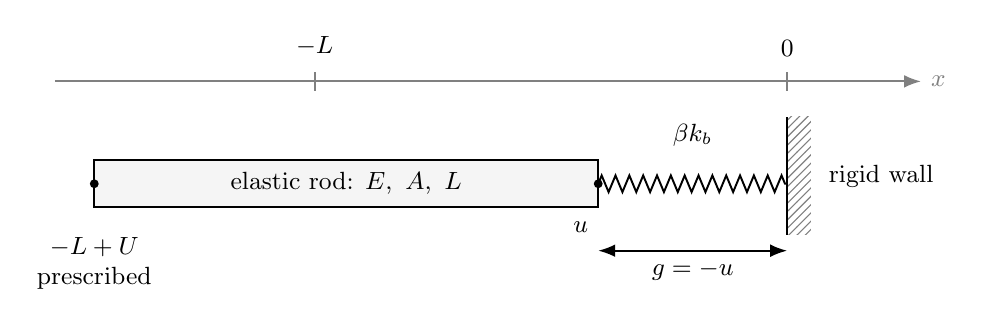
\begin{tikzpicture}[>=Latex,font=\small,line width=0.7pt]
  \draw[->,gray] (0,1.35) -- (11,1.35) node[right] {$x$};
  \draw[gray] (3.3,1.23) -- (3.3,1.47) node[above=2pt,black] {$-L$};
  \draw[gray] (9.3,1.23) -- (9.3,1.47) node[above=2pt,black] {$0$};
  \draw[fill=gray!8] (0.5,-0.25) rectangle (6.9,0.35);
  \node at (3.7,0.05) {elastic rod: $E,\ A,\ L$};
  \fill (0.5,0.05) circle (1.6pt);
  \fill (6.9,0.05) circle (1.6pt);
  \draw[decorate,decoration={zigzag,segment length=5pt,amplitude=3pt}]
    (6.9,0.05) -- (9.3,0.05);
  \node[above] at (8.1,0.4) {$\beta k_b$};
  \fill[pattern=north east lines,pattern color=gray] (9.3,-0.6) rectangle (9.6,0.9);
  \draw[thick] (9.3,-0.6) -- (9.3,0.9);
  \node[right] at (9.7,0.15) {rigid wall};
  \draw[<->] (6.9,-0.8) -- (9.3,-0.8) node[midway,below] {$g=-u$};
  \node[below,align=center] at (0.5,-0.5) {$-L+U$\\prescribed};
  \node[below left] at (6.9,-0.3) {$u$};
\end{tikzpicture}
\caption{An opened configuration, not to scale. A positive gap is compatible
with surviving adhesion. Compressive contact acts at zero gap and is not scaled
by the active bond fraction.}
\end{figure}

The rod is homogeneous, small-strain, linear elastic, and uniaxial, not a
plane-strain reduction. Body forces, inertia, creep, plasticity, friction,
tangential motion, diffusion, and temperature evolution are omitted. With
displacement field $w$, its strain and tension-positive force are
\begin{equation}
 \varepsilon=w_{,x}=\frac{u-U}{L},\qquad
 N=EA\varepsilon=k_r(u-U),\qquad k_r=\frac{EA}{L}.
\end{equation}
Let $K_n\geq0$ be fully bonded interface stiffness per area, with stress per
length units, and $k_b=AK_n$ the corresponding force per length stiffness.
The attractive spring force is $F_b=\beta k_b g$. The wall's compressive
reaction has magnitude $P$ and acts in the opposite direction:
\begin{equation}
 N=F_b-P,\qquad P\geq0,\quad g\geq0,\quad Pg=0.
 \label{eq:contact}
\end{equation}
The actuator force on the left node is $-N$; the code reports $N$.

For virtual displacements with $\delta w(-L)=0$, the weak equation is
\begin{equation}
 \int_{-L}^{0}EA w_{,x}\delta w_{,x}\,\dd x-(F_b-P)\delta w(0)=0.
\end{equation}
Linear shape functions give the stiffness
$k_r\begin{bmatrix}1&-1\\-1&1\end{bmatrix}$ and the reduced residual
$[k_r(u-U)-F_b+P]\delta u=0$. One-point quadrature integrates the constant
rod stiffness exactly. With no body force, this linear element also represents
the exact axial equilibrium displacement.

For $U>0$, contact gives $g=u=F_b=0$ and $P=k_rU$. For $U<0$, a contacting
tip would require a negative reaction, so $P=0$ and
$(k_r+\beta k_b)g=-k_rU$. Both branches are
\begin{equation}
 \boxed{P=k_r\pos{U},\quad g=\frac{\pos{-U}}{1+r\beta},\quad
 u=-g,\quad F_b=\beta k_b g,\quad N=F_b-P,\quad r=\frac{k_b}{k_r}.}
 \label{eq:mechanics}
\end{equation}
Here $\pos{z}=\max(z,0)$. The denominator is positive on the admissible
domain. No penalty, multiplier iteration, or numerical contact stiffness is
introduced; the physical contact reaction has been condensed analytically.

\subsection{Measured stress versus surviving-bond loading}

Pressure and nominal tensile traction use the full area, while surviving-bond
traction uses the active portion under the uniform load-sharing assumption:
\begin{equation}
 p=\frac{P}{A},\qquad \sigma=\frac{F_b}{A}=\pos{N/A}=\beta K_n g,
 \qquad \tau=\frac{\sigma}{\beta}=K_ng\quad(\beta>0).
 \label{eq:tractions}
\end{equation}
The code calls these \code{pressure}, \code{traction}, and
\code{bond_traction}, respectively. It evaluates $\tau=K_ng$ directly, never
by dividing by a small $\beta$. At $\beta=0$ this expression is a limiting
trial demand, not an actual stress on nonexistent bonds: nominal force and
bond loss are zero. A diagnostic can omit such states from a logarithmic plot
without changing the stored arrays or imposing a failure cutoff.

This choice retains a linear spring and a single history variable. It is
mathematically a stress-scaled gap driver, since $K_n$ is constant; changing
the terminology alone does not add microscopic physics. The meaningful change
from a fixed nominal-stress switch is that the decreasing active fraction no
longer reduces the quantity used to activate rupture.

\section{Formation, rupture, and unloading}

Physical time remains essential despite quasistatic mechanical equilibrium.
The competing rates are
\begin{equation}
 \dot\beta=a(1-\beta)-b\beta,\qquad
 a=k_f\frac{p}{p_{\mathrm{ref}}},\qquad b=k_d S_b(\tau).
 \label{eq:kinetics}
\end{equation}
Both rate constants are nonnegative and have inverse-time units, and
$p_{\mathrm{ref}}>0$. The switch is
\begin{equation}
 S_b(\tau)=\begin{cases}
 0,&\tau\leq\tau_0,\\
 3z^2-2z^3,&\tau_0<\tau<\tau_0+\Delta\tau,\\
 1,&\tau\geq\tau_0+\Delta\tau,
 \end{cases}
 \qquad z=\frac{\tau-\tau_0}{\Delta\tau}.
 \label{eq:switch}
\end{equation}
The parameters \code{bond_sigma0} and \code{bond_delta_sigma} denote
$\tau_0\geq0$ and $\Delta\tau>0$. They are \emph{bonded-area stress scales},
not nominal strength values. The width is a constitutive parameter, independent
of the time-step size. The switch and its first derivative are continuous.
There is no additional power multiplier, baseline rupture rate, permanent
activation flag, or independent cohesive damage law.

In contact $g=\tau=0$, so only formation acts. In opening $p=0$, so only
rupture can act. At $\beta=0$, the rate is $a\geq0$; at $\beta=1$, it is
$-b\leq0$. These signs preserve the continuous interval $[0,1]$.
The existence of a gap does not alone imply loss: its bonded-area demand must
exceed the onset threshold.

\subsection{Why falling nominal traction does not stop an activated hold}

Fix the actuator at $U=-G<0$. From Eq.~\eqref{eq:mechanics},
\begin{equation}
 g=\frac{G}{1+r\beta},\quad
 \sigma=\frac{\beta K_nG}{1+r\beta},\quad
 \tau=\frac{K_nG}{1+r\beta},\quad
 \frac{\dd\sigma}{\dd\beta}=\frac{K_nG}{(1+r\beta)^2},\quad
 \frac{\dd\tau}{\dd\beta}=-\frac{rK_nG}{(1+r\beta)^2}.
 \label{eq:feedback}
\end{equation}
As bonds disappear, the gap grows and the rod unloads. The measured nominal
traction decreases, but surviving-bond traction increases. If the switch was
already active, it cannot become inactive during that fixed-actuator hold.
Once fully activated it remains fully activated, without storing an extra flag.
Then the continuous solution is
\begin{equation}
 \beta(t)=\beta(t_*)\exp[-k_d(t-t_*)].
 \label{eq:exponential}
\end{equation}
More generally, an initially positive switch value bounds the subsequent loss
rate away from zero during the hold, so $\beta$, nominal force, and rod strain
approach zero when $k_d>0$. A positive fraction does not reach exactly zero in
finite time at bounded rates, apart from eventual floating-point underflow.
There is no positive arrest fraction caused by falling nominal stress.

This does not mean every experiment must debond. A subthreshold held state is
stationary. Deliberately decreasing $G$ can unload surviving bonds and stop
further loss; existing loss is not undone. After compressive recontact,
formation can rebuild $\beta$. This distinction is why the model does not
permanently latch the switch. It is also why merely looping an animation is
not equivalent to simulating additional physical loading cycles.

\subsection{Pressure exposure, strength, and energy}

During compression, the exact continuous formation result is
\begin{equation}
 \beta_{\mathrm{end}}=1-(1-\beta_{\mathrm{start}})
 \exp\left[-\frac{k_f}{p_{\mathrm{ref}}}\int p(t)\,\dd t\right].
 \label{eq:dose}
\end{equation}
Loading and unloading ramps contribute alongside the pressure hold. Thus the
baseline combines pressure and time through integrated exposure rather than
two independent microscopic mechanisms. Formation identifies the ratio
$k_f/p_{\mathrm{ref}}$ unless one factor is specified independently.
Before opening loss starts, an active fraction $\beta_b$ gives nominal onset
$\sigma_{\mathrm{onset}}=\beta_b\tau_0$. The nominal onset therefore scales
with the amount of bonding; it is not a fixed threshold independent of the
pressure/hold history. The later force peak also depends on loading speed,
compliance, and kinetics, so onset is not a hard maximum-strength cap.

The elastic interface energy per nominal area provides a useful sign check:
\begin{equation}
 \psi_{\mathrm{int}}=\tfrac12\beta K_ng^2,\qquad
 \partial_g\psi_{\mathrm{int}}=\sigma,\qquad
 \mathcal D_{\mathrm{loss}}=-\tfrac12K_ng^2\dot\beta\geq0.
\end{equation}
Formation acts at $g=0$ and therefore adds no elastic spring energy in this
idealization. This is not a chemical thermodynamic proof: chemical free energy,
diffusion, and temperature dependence have not been specified. The law also
does not prescribe a calibrated fracture energy. For quantitative copper
predictions, full load histories, work of separation, failure location, and
possible bulk inelasticity need experimental assessment.

\section{The experiment and its parameters}

Every cycle begins at $U=-D$ and ends at the same actuator coordinate. In
contact the target displacement is $U_{\mathrm{press}}=p_{\mathrm{peak}}L/E$.
The pull duration is $D/v_{\mathrm{pull}}$, independent of peak pressure.
Separating compression unloading from tensile pulling avoids inadvertently
changing tensile speed when pressure is varied.

\begin{table}[htbp]
\centering\small
\caption{The piecewise-linear loading protocol; zero-duration holds are omitted.}
\begin{tabularx}{\linewidth}{@{}l l Y@{}}
\toprule
Phase & Duration & Prescribed motion or hold\\
\midrule
Approach / return & $t_{\mathrm{approach}}$ & $-D\longrightarrow0$\\
Press & $t_{\mathrm{press}}$ & $0\longrightarrow U_{\mathrm{press}}$\\
Compressed hold & $t_{\mathrm{hold}}$ & $U=U_{\mathrm{press}}$\\
Unload compression & $t_{\mathrm{unload}}$ & $U_{\mathrm{press}}\longrightarrow0$\\
Tensile pull & $D/v_{\mathrm{pull}}$ & $0\longrightarrow-D$\\
Open-actuator hold & $t_{\mathrm{open\,hold}}$ & $U=-D$\\
\bottomrule
\end{tabularx}
\end{table}

The next approach is a return of the same interface. Its surviving bonds can
still rupture while sufficiently stretched; pressure-driven formation begins
only after contact is restored. No state is reset at the cycle boundary.
Conversely, each \emph{independent sweep case} starts from the same specified
$\beta_0$. Its pressure dose per cycle is
\begin{equation}
 Q_p=p_{\mathrm{peak}}\left(t_{\mathrm{press}}/2+t_{\mathrm{hold}}
                                      +t_{\mathrm{unload}}/2\right).
\end{equation}
Equation~\eqref{eq:dose} applies to the compression interval starting with the
fraction after approach, not to an entire cycle that also includes rupture.

\begin{table}[htbp]
\centering\small
\caption{Module defaults. All units are internally consistent but arbitrary;
no value is a measured copper property. Stress is force per area.}
\begin{tabularx}{\linewidth}{@{}l r Y@{}}
\toprule
Input & Default & Meaning / units\\
\midrule
\code{E}, \code{A}, \code{L} & $100,1,1$ & Modulus [stress], area, length\\
\code{K_n} & $10$ & Fully bonded stiffness [stress/length]\\
\code{k_f}, \code{p_ref} & $1,0.1$ & Formation rate [1/time], pressure scale [stress]\\
\code{k_d} & $1$ & Fully activated rupture rate [1/time]\\
\code{bond_sigma0} & $0.04$ & Bonded-area onset $\tau_0$ [stress]\\
\code{bond_delta_sigma} & $0.02$ & Bonded-area activation width $\Delta\tau$ [stress]\\
\code{beta0}, \code{p_peak} & $0,0.1$ & Initial fraction, peak pressure [stress]\\
\code{t_approach}, \code{t_press} & $1,1$ & Ramp durations [time]\\
\code{t_hold}, \code{t_unload} & $3,1$ & Compressed hold and unload durations [time]\\
\code{pull_distance}, \code{v_pull} & $0.12,0.04$ & Retraction [length], speed [length/time]\\
\code{t_open_hold}, \code{cycles} & $3,1$ & Open hold [time], number of physical cycles\\
\code{dt} & $0.03$ & Maximum internal step and output spacing [time]\\
\code{rtol}, \code{atol} & $10^{-5},10^{-9}$ & Relative and absolute beta error scales\\
\bottomrule
\end{tabularx}
\end{table}

All inputs and derived scales must be finite. Modulus, area, length, pressure
scale, activation width, non-hold durations, pull distance and speed, and
numerical step/tolerance scales are positive. Rates, interface stiffness,
onset, peak pressure, and hold durations may be zero but not negative.
The fraction lies in $[0,1]$ and the cycle count is a positive integer.
The code rejects $p_{\mathrm{peak}}\geq E$ to avoid rod inversion, but the
actual small-strain requirement is much stronger: $|N|/(EA)\ll1$ throughout
the history. A large actuator travel can mainly become gap rather than rod
strain. Area scaling is explicit: changing $A$ scales forces and both total
stiffnesses together, leaving the stress-driven beta trajectory unchanged.

The notebook's \emph{Visible Stickiness} preset uses $E=5$, $K_n=250$,
$p_{\mathrm{peak}}=p_{\mathrm{ref}}=0.05$, $\tau_0=0.02$,
$\Delta\tau=0.01$, $k_d=2$, $D=0.08$, and $v_{\mathrm{pull}}=0.015$.
The compressed and open holds are $4$ and $8$ time units; it uses one cycle
and $\code{dt}=0.01$, with other inputs unchanged. These explicitly
bonded-area thresholds are not a conversion of earlier nominal-strength data.
The stiffness ratio is $50$: with beta near one, only about $1/51$ of initial
retraction moves the tip, making elastic stretching easier to see. The default
pressure sweep ends at $0.1$, limiting its compression strain to two percent.

\section{Implicit integration without spurious rupture}

\subsection{Residual, derivative, and the uniqueness safeguard}

After mechanical condensation, only beta requires integration. Backward Euler
at a prescribed endpoint $U_{n+1}$ gives
\begin{equation}
 R(\beta)=\beta-\beta_n-ha(1-\beta)+h b(\tau(\beta))\beta=0.
 \label{eq:be}
\end{equation}
In compression $b=0$ and the exact solution of this \emph{discrete} equation
is $(\beta_n+ha)/(1+ha)$. This is not the exact continuous formation
exponential. In opening, $a=0$, and for $G=-U_{n+1}>0$,
\begin{equation}
 R'(\beta)=1+hb-h\beta b_\tau\frac{r\tau}{1+r\beta},\qquad
 b_\tau=\frac{6k_dz(1-z)}{\Delta\tau}
 \quad\hbox{inside the switch interval}.
 \label{eq:derivative}
\end{equation}
Outside the interval $b_\tau=0$. The negative term is the mechanical feedback
of increasing surviving-bond demand. Unlike a nominal-stress gate, a large
opening step can therefore make the residual nonmonotone.

The code first handles stationary and fully activated branches. If the old
fraction evaluated at the new actuator position is subthreshold, it retains
that stationary branch instead of selecting a spurious large-step damaged
root. If it is fully activated, every smaller fraction is also fully active,
and the unique update is $\beta_n/(1+hk_d)$. A zero old fraction remains zero
during opening without division. These are exact discrete branch solutions.

For a partially activated old state, define $T=K_nG$ and
\begin{equation}
 B=\frac{r\beta_n}{1+r\beta_n}\,
       \min(T,\tau_0+\Delta\tau)\,\frac{1.5k_d}{\Delta\tau}.
 \label{eq:bound}
\end{equation}
This bounds $\beta b_\tau|\dd\tau/\dd\beta|$ throughout $[0,\beta_n]$:
the fractional prefactor increases with beta, the switch slope is at most
$1.5k_d/\Delta\tau$, and wherever that slope is nonzero the traction is at
most $\min(T,\tau_0+\Delta\tau)$. Requiring $hB\leq0.8$ gives
$R'\geq0.2$. Since $R(0)=-\beta_n$ and $R(\beta_n)\geq0$, this guarantees
one root in the admissible decay bracket. The factor $0.8$ is a dimensionless
solver safety margin, not material damping or a constitutive parameter.

To retain relative accuracy for tiny fractions, solve $q=\beta/\beta_n$:
\begin{equation}
 H(q)=q[1+h b(\tau(\beta_nq))]-1=0,\qquad 0\leq q\leq1.
\end{equation}
Its analytic derivative follows from
$\tau_q=-r\beta_n\tau/(1+r\beta_nq)$. Safeguarded Newton proposals outside
the central 80 percent of the current bracket are replaced by bisection.
A failed uniqueness bound or scalar solve rejects the trial; it never clips
beta or commits an unconverged iterate. The continuous stationary solution
and the guarded discrete root must not be confused with choosing an arbitrary
root of an unrestricted large-step equation.

\subsection{Time accuracy and reproducibility across cycles}

Adaptive step doubling compares one full BE step with two consecutive half
steps from the same accepted state, using the actuator value at each step's
own endpoint. The normalized error is
\begin{equation}
 e=\frac{|\beta_{\mathrm{two}}-\beta_{\mathrm{full}}|}
 {\code{atol}+\code{rtol}\max(\beta_n,\beta_{\mathrm{two}})}.
\end{equation}
If $e\leq1$, the two-half-step result is accepted; no Richardson extrapolation
is used because it need not preserve bounds. Rejected trials advance neither
time nor state. The scheme remains first order globally. A local error
tolerance is not a guarantee on the final history or sampled peak stress.

All load corners are output events and internal steps do not cross them.
Integration uses phase-local time and the exact input phase duration, so
shifting the same cycle to a later absolute time does not change adaptive
decisions through cancellation in endpoint subtraction. Stored output times
are then shifted to the global timeline, retaining exact phase endpoints.
The code validates representable output spacing and limits outputs to 200,000
points, adaptive trials to 2,000,000, and independent sweep cases to 128.
Exceeding a resource or representability limit is reported, not silently
shortened or regularized.

\section{Reading and verifying the notebook}

The frozen \code{Parameters} object defines one run. \code{load_segments}
records cycle, phase, start, end, duration, and the two endpoint displacements.
\code{simulate} returns the accepted arrays and step statistics;
\code{summarize_cycles} reports nominal peak stress, its time, initial and
final fractions, pressure dose, and equilibrium/complementarity errors.
The peak is taken during tensile pulling and its following open hold, not
during the next return. A shared boundary sample belongs to the preceding
phase label, so summaries use inclusive time bounds rather than labels alone.
The \code{peak_at_pull_end} flag marks a positive maximum at the prescribed
pull endpoint. It is potentially range-limited, not proven pull-off strength.

\code{sweep} varies only peak pressure or compressed hold time, starting each
case independently from the same initial fraction and carrying history within
any subsequent physical cycles. Peak stress always means nominal stress,
never the much larger bonded-area demand. The diagnostic panels show both
measures separately. A constant bonded-area threshold must not be overlaid
as a constant nominal-strength line; the equivalent nominal onset is
$\beta\tau_0$ and changes with the active fraction.

The animation consumes an already computed trajectory. It interpolates $U$
and beta in physical time, recomputes mechanics, and only then applies a
display-only magnification $s\geq1$:
\begin{equation}
 x_{\mathrm{left}}^{\mathrm{display}}=-L+sU,\qquad
 x_{\mathrm{tip}}^{\mathrm{display}}=su,\qquad
 L_{\mathrm{rod}}^{\mathrm{display}}=L+s(u-U).
\end{equation}
The default notebook factor is $10$; $1$ restores actual geometry. A dashed
unstretched-length guide follows the actuator. It is not a second rod and
may cross the wall during compression. Numeric strain, gap, pressure, and
both traction labels remain physical, as do all history plots. A magnification
that collapses the displayed compressed rod is rejected. Adhesive opacity
tracks beta continuously, with no visual failure cutoff. The initial movie
uses 120 frames at 5 fps, about 24 seconds for one cycle. The loop button
replays that trajectory; changing the physical cycle count is a separate action.

Regression tests check mechanical equilibrium, contact complementarity,
switch and residual derivatives by centered differences, stationary and fully
activated branches, the uniqueness safeguard, tiny fractions, area scaling,
and invalid inputs. In particular, an activated fixed-actuator hold must
continue losing bonds while nominal traction decreases, following the
exponential oracle once fully active. Closure must be able to stop loss and
compression must permit formation without an activation reset. Cycle-by-cycle
and continuous runs must agree; sweep values must not inherit each other's
history. Time refinement checks histories and nominal peaks, not just force
balance. Animation tests distinguish physical mechanics from display scaling.

These are implementation checks, not experimental validation. The notebook
retains executed results, exact parameters, dependency versions, and a source
hash. This document explains the assumptions and algorithms rather than
exporting simulation results. The README contains setup and launch instructions.

\begin{thebibliography}{9}
\bibitem{designhistory}
\emph{Formulate Weak Form}. Shared ChatGPT conversation, design history.
Accessed 6 September 2026.
\url{https://chatgpt.com/share/6a9dc146-1d1c-83e8-bbb7-e159d93ad7c8}.
Used for the minimal rod/contact model, the nonfailing spring requirement,
and the evolution of candidate drivers; not physical validation.
\bibitem{erdmann2004}
T.~Erdmann and U.~S.~Schwarz, ``Stability of Adhesion Clusters under Constant
Force,'' \emph{Physical Review Letters} \textbf{92}, 108102 (2004).
\href{https://doi.org/10.1103/PhysRevLett.92.108102}{doi:10.1103/PhysRevLett.92.108102}.
Figure~1 is used for uniform sharing among closed bonds; its biological
constant-force off-rate is not adopted as the present copper interface law.
\end{thebibliography}
\end{document}
